% !TEX encoding = UTF-8
% !TEX TS-program = pdflatex
% !TEX root = ../tesi.tex

%**************************************************************
\section{Sprint 4}
\label{sec:sprint4}
%**************************************************************

\subsection{User stories assegnate}
\paragraph{Filtri utente, cliente, progetto e task (rispettivamente 5, 2, 2 e 2)}\mbox{} \\[\baselineskip]
\noindent Come utente autenticato che si trova nella sezione “Reports”, voglio poter scegliere uno o più utenti, clienti, progetti o task, anche contemporaneamente, e visualizzare le ore lavorative spese dall'utente o dedicate al cliente/progetto/task.\\

\noindent Tasks:

\begin{itemize}
  \item Implementare il componente dei filtri;
  \begin{itemize}
    \item implementare il componente principale;
    \item implementare lo stile per i filtri;
  \end{itemize}
  \item Implementare la logica di query nel backend per i filtri.
\end{itemize}

\subsection{Filtri utente, cliente, progetto e task}
\noindent A ciò che ho già fatto, è richiesto di aggiungere una toolbar, posizionata sopra la tabella, che permetta all'utente, tramite dei menù a tendina, di filtrare i dati che vengono mostrati, in particolare utenti, clienti, progetti e task. \\
Innanzitutto ho creato il component principale \texttt{ReportFilter} contenente la toolbar e i vari filtri. \\
Per creare elementi grafici come input, select, button ho utilizzato una libreria grafica React già utilizzata nel resto della applicazione: MUI\footcite{site:mui}. In questo modo, oltre a mantenere una consistenza di stile con il resto della app, è risultato più facile interagire con questi elementi grafici (come tenere traccia di quali elementi sono selezionati nei select).\\
Successivamente, erano necessarie delle nuove richieste al backend per ottenere le liste di tutti gli utenti, clienti, progetti e task da mostrare nei rispettivi filtri. I vari endpoint erano già presenti, non ho quindi dovuto ancora toccare il backend per le richieste.\\
Avendo tutti i dati necessari, è stato sufficiente renderli disponibili al component principale \texttt{Reports} in modo da poterli usare nella richiesta per i dati già implementata. In particolare ho aggiunto i seguenti queryparams:
\begin{itemize}
  \item \texttt{users}: un array contenente gli utenti selezionati nei filtri;
  \item \texttt{clients}: un array contenente i clienti selezionati nei filtri;
  \item \texttt{projects}: un array contenente i progetti selezionati nei filtri;
  \item \texttt{tasks}: un array contenente i task selezionati nei filtri.
\end{itemize}
Ho modificato il backend di conseguenza, in modo che la query già implementata ottenesse solo le attività con, ad esempio, il campo \texttt{task} uguale a uno degli elementi presenti nell'array \texttt{tasks}. Con MongoDB questa è un'operazione piuttosto semplice in quanto basta utilizzare la keyword \texttt{\$match} che permette appunto di ottenere documenti che rispettano una condizione, come mostrato nell'esempio di codice \ref{code:mongo}.

\begin{code}[frame=tb, label={code:mongo}, caption={Esempio di filtro task lato backend con MongoDB}]\\
1  {
2    $match: tasks
3    ? { task: { $in: tasks } }
4    : { task: { $exists: true } },
5  },
\end{code}\\\\

\noindent In questo caso, se l'utente ha selezionato almeno un task, verrà eseguita la linea 3 del codice ottenendo solo i documenti con il campo \texttt{task} che compare in \texttt{tasks}, altrimenti verranno ottenuti tutti i documenti (linea 4).

\subsection{Sprint review}
La sprint review si è conclusa in modo positivo, senza particolari correzioni necessarie.
Anche i tempi sono stati rispettati.\\
Nella figura \ref{fig:report_filters} sono visibili i filtri realizzati, posizionati sopra la tabella.

\begin{figure}[H]
	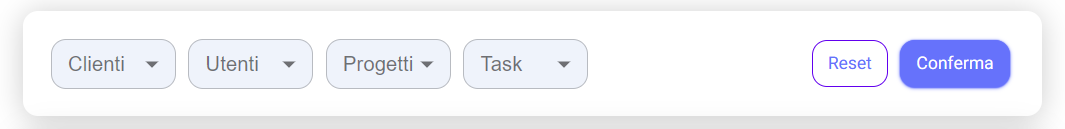
\includegraphics[width = \textwidth]{immagini/reports filters.png}
	\caption{Filtri della tabella}
	\label{fig:report_filters}
\end{figure}